\documentclass[a4paper, titlepage]{article}
\usepackage[round, sort, numbers]{natbib}
\usepackage[utf8]{inputenc}
\usepackage{amsfonts, amsmath, amssymb, amsthm}
\usepackage{color}
\usepackage{listings}
\usepackage{mathtools}
\usepackage{marvosym}
\usepackage{paralist}
\usepackage{parskip}
\usepackage{subfig}
\usepackage{tikz}
\usepackage{titlesec}

\numberwithin{figure}{section}
\numberwithin{table}{section}

\usetikzlibrary{arrows, automata, backgrounds, petri, positioning}
\tikzstyle{place}=[circle, draw=blue!50, fill=blue!20, thick]
\tikzstyle{marking}=[circle, draw=blue!50, thick, align=center]
\tikzstyle{transition}=[rectangle, draw=black!50, fill=black!20, thick]

% define new commands for sets and tuple
\newcommand{\setof}[1]{\ensuremath{\left \{ #1 \right \}}}
\newcommand{\tuple}[1]{\ensuremath{\left \langle #1 \right \rangle }}
\newcommand{\card}[1]{\ensuremath{\left \vert #1 \right \vert }}

\makeatletter
\newcommand\objective[1]{\def\@objective{#1}}
\newcommand{\makecustomtitle}{%
	\begin{center}
		\huge\@title \\
		[1ex]\small Aurélien Coet, Dimitri Racordon
	\end{center}
	\@objective
}
\makeatother

\begin{document}

\title{Outils formels de Modélisation \\ 7\textsuperscript{ème} séance d'exercices}
\author{Aurélien Coet, Dimitri Racordon}
\objective{
Dans cette séance d'exercices, nous allons étudier l'algèbre linéaire dans le cadre des réseaux de Petri.
}

\makecustomtitle

\section{Producteur/consommateur [\Keyboard] ($\bigstar$)}
Considérez le réseau de la figure \ref{fig:robots}, lequel représente un modèle \emph{producteur consommateur}.
\begin{enumerate}
  \item Calculez la matrice représentant sa fonction d'entrée et celle représentant sa fonction de sortie. Déduisez-en sa \emph{matrice d'incidence}.
  \item Représentez son marquage initial $M_0$ en notation vectorielle.
  \item En utilisant ces matrices, calculez le résultat du tir de la séquence de transition $t_0 \rightarrow t_1 \rightarrow t_0 \rightarrow t_1 \rightarrow t_2$.
  \item Dans le fichier \texttt{Program.fs} du projet \texttt{Exercise}, construisez la matrice d'incidence du réseau, puis utilisez cette dernière pour calculer le résultat du tir de la séquence de transitions $t_0 \rightarrow t_1 \rightarrow t_0 \rightarrow t_1 \rightarrow t_0 \rightarrow t_1 \rightarrow t_2 \rightarrow t_3$ depuis le marquage initial.
  \item De la même manière, calculez le résultat du tir de la séquence de transition $t_0 \rightarrow t_1 \rightarrow t_2 \rightarrow t_3 \rightarrow t_2$.
\end{enumerate}

\begin{figure}[ht]
	\centering
  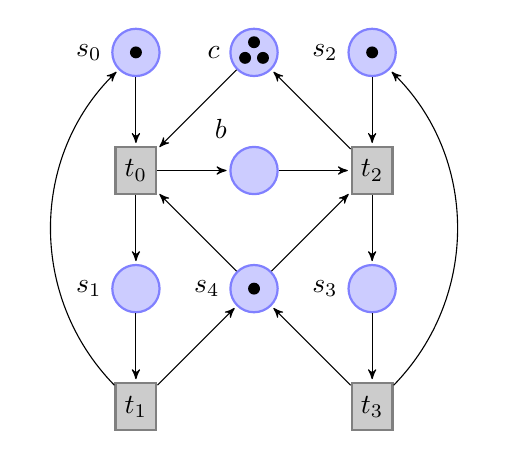
\begin{tikzpicture}[node distance=1.5cm, minimum height=6mm, >=stealth', bend angle=45, auto]
    \node[place,tokens=1] (s0) [label=left:$s_0$] {};
    \node[place] (s1) [below of=s0, yshift=-1.5cm, label=left:$s_1$] {};

    \node[place,tokens=3] (cb) [right of=s0, label=left:$c$] {};
    \node[place] (b) [below of=cb, label=135:$b$] {};
    \node[place,tokens=1] (s4) [below of=b, label=left:$s_4$] {};

    \node[place,tokens=1] (s2) [right of=cb, label=left:$s_2$] {};
    \node[place] (s3) [below of=s2, yshift=-1.5cm, label=left:$s_3$] {};

    \node [transition] (t0) [below of=s0] {$t_0$}
				  edge [pre] (s0) edge [pre] (cb) edge [pre] (s4)
          edge [post] (b) edge [post] (s1);
    \node [transition] (t1) [below of=s1] {$t_1$}
				  edge [pre] (s1)
          edge [post,bend left] (s0) edge [post] (s4);

    \node [transition] (t2) [below of=s2] {$t_2$}
				  edge [pre] (s2) edge [pre] (s4) edge [pre] (b)
          edge [post] (cb) edge [post] (s3);
    \node [transition] (t3) [below of=s3] {$t_3$}
				  edge [pre] (s3)
          edge [post,bend right] (s2) edge [post] (s4);
  \end{tikzpicture}
	\caption{Un modèle producteur/consommateur}
	\label{fig:robots}
\end{figure}

\clearpage

\section{Salut Bézout! [\Keyboard] ($\bigstar\bigstar$)}
Considérez le réseau de la figure \ref{fig:bezout}.

\begin{enumerate}
  \item Donnez le vecteur caractéristique de la séquence de transitions suivante: $t_0 \rightarrow{} t_1 \rightarrow{} t_0 \rightarrow{} t_0 \rightarrow{} t_2 \rightarrow{} t_3 \rightarrow{} t_2 \rightarrow{} t_1 \rightarrow{} t_4 \rightarrow{} t_3 \rightarrow{} t_2 \rightarrow{} t_4$
  \item Sachant que cette séquence de transitions est tirable, donnez le marquage obtenu après son tir.
  \item Est-il possible pour ce réseau de revenir au marquage initial Après avoir tiré au moins une fois la transition $t_0$? Si oui, combien de fois devrait-on tirer $t_4$ au minimum pour que ça arrive?
  \item Est-il possible pour ce réseau d'atteindre le marquage $\tuple{1,0,0,0,3}$? Si oui, combien de fois devrait-on tirer la transition $t_4$ au minimum pour que ça arrive?
\end{enumerate}

\begin{figure}[ht]
  \centering
    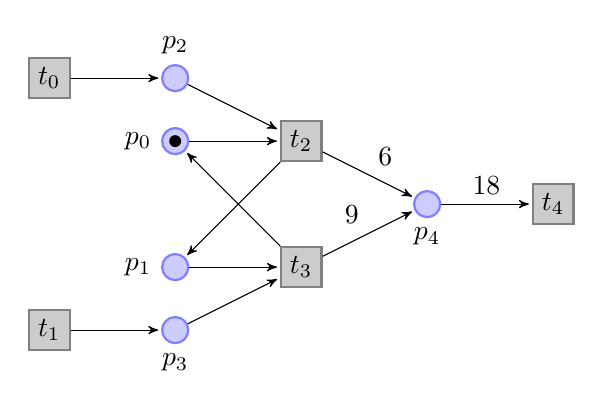
\begin{tikzpicture}[node distance=16mm, >=stealth', bend angle=45, auto]
      \node[place] (p4) [label=below:$p_4$] {};
      \node[place,tokens=1] (p0) [left of=p4,xshift=-16mm,yshift=8mm,label=left:$p_0$] {};
      \node[place] (p1) [left of=p4,xshift=-16mm,yshift=-8mm,label=left:$p_1$] {};
      \node[place] (p2) [above of=p0,yshift=-8mm,label=above:$p_2$] {};
      \node[place] (p3) [below of=p1,yshift=8mm,label=below:$p_3$] {};

      \node [transition] (t0) [left of=p2] {$t_0$}
            edge [post] (p2);
      \node [transition] (t1) [left of=p3] {$t_1$}
            edge [post] (p3);
      \node [transition] (t2) [right of=p0] {$t_2$}
            edge [pre] (p0)
            edge [pre] (p2)
            edge [post] node {6} (p4)
            edge [post] (p1);
      \node [transition] (t3) [right of=p1] {$t_3$}
            edge [pre] (p1)
            edge [pre] (p3)
            edge [post] node {9} (p4)
            edge [post] (p0);
      \node [transition] (t4) [right of=p4] {$t_4$}
            edge [pre] node[swap] {18} (p4);
    \end{tikzpicture}
	\caption{Réseau exposant des propriétés algébriques intéressantes}
	\label{fig:bezout}
\end{figure}

\end{document}
